%% Written 2026-11-12 from the run records of the JFNK -> march -> JFNK
%% experiment; every number is measured by the scripts in
%% scratch_jfnk_from_marching_20261111/heh0p1_s2p53/remarch/analysis/.
%% Author: Kwang-Il Seon
\documentclass[english,a4paper]{my_memo}
\synctex=1
\usepackage{amsmath}
\usepackage{amssymb}
\usepackage{booktabs}
\usepackage{array}
\usepackage{url}
\urlstyle{tt}
\usepackage{babel}
\usepackage[section]{placeins}
\newcommand{\ev}[1]{\textnormal{\small[#1]}}
\newcommand{\Rp}{R_p}
\sloppy
\begin{document}

\title{JFNK, marching, and JFNK again from one molecular LHS~1140\,b state
(He/H 0.1, $s=2.53$)}
\author{Kwang-Il Seon}
\maketitle

\section*{Summary}

\textbf{Verdict.} Neither JFNK attempt produced a stationary state, and marching
the first JFNK last iterate did not bring it back to the marching state
within the 31\,311\,s (0.106 flow-crossing times) that were marched. Some
differences decreased (the largest density difference from 0.226 to
0.199\,dex), but an overall return was not observed. The two attempts show
similar late-pass diagnostics, especially in passes 36--48. Their
uncertified last iterates have opposite helium-rich and helium-poor
distributions and differ strongly from each other and from the campaign
state.
\begin{itemize}
\item \textbf{JFNK-1} (from chunk~61) and \textbf{JFNK-2} (from the end of
the remarch): 60 outer passes each, \texttt{info=1}, exit status~3,
certified=F. The reported hydrodynamic rows of the retained wind remain
small (mass $\le6.3\times10^{-8}$, momentum $\le3\times10^{-11}$, energy
$\le1.6\times10^{-8}$); four hydrodynamic solves fail and restore an earlier
converged wind (Section~\ref{sec:c}). Meanwhile the worst carrier row measured after that solve
stays at 0.42--1.0 against $10^{-5}$ from pass~9 (JFNK-1) and pass~2
(JFNK-2) on.
\item \textbf{A (carriers).} When the JFNK-1 iterate is marched, H$_2^+$,
H$_3^+$ and HeH$^+$ at 1.2--1.5\,$\Rp$ fall by 0.40--1.03\,dex by the
first frame (1564.5\,s) and He$^+$, He(2$^3$S) rise by 0.16--0.36\,dex at
1.27--2\,$\Rp$; H$^+$ and $e^-$ in the layer (1.03--1.5\,$\Rp$) then change by
0.3--0.75\,dex, together with an inflow that develops at
1.03--1.13\,$\Rp$. At selected cells these later changes reach half of their
measured log-density change after 6000--8500\,s. The carriers evolve in the
displaced fluid and helium distribution; they have not returned to the
chunk-61 values, and some still change during the last chunk.
\item \textbf{B (fluid).} Against the campaign at equal elapsed time, the
largest density difference goes from 0.226 to 0.199\,dex (rms 0.082 to
0.083\,dex), the temperature difference from 0.075 to 0.071\,dex, and the
velocity measure grows from 0.09 to 0.42: some differences decrease, but
no overall return is observed. A persistent difference is the helium
distribution of the JFNK-1 uncertified last iterate, with local He/H up to
13 times the campaign value, in a layer whose advection times exceed
$10^6$\,s.
\item \textbf{C, D.} JFNK-2 moves its start by up to 0.41\,dex in $\rho$ and
removes helium from the wind (He/H $1.5\times10^{-11}$ at $10\,\Rp$), the
opposite of JFNK-1 (0.045); its $4\pi\rho v r^2$ is $1.87\times10^8$\,g\,s$^{-1}$
against $7.08\times10^7$ (JFNK-1) and $7.28\times10^7$ (chunk~61). The two adjacent
saved pass states of each attempt have opposite helium-poor and
helium-rich wind distributions. Similar scalar pass diagnostics do not
establish repetition of the full states; the displacement is not
reproducible as a state.
\item \textbf{E.} The composition update at fixed wind can reduce the
worst carrier row to $5\times10^{-5}$ (still above $10^{-5}$), but the next
hydrodynamic solve, with transported fractions retained and the usual
thermochemical and boundary refreshes applied, raises it to 0.55--1.0 in
the listed passes; the march holds them at
$10^{-4}$--$2\times10^{-2}$ (H$_2$ up to 0.15). The records appear consistent with a partitioned
iteration that does not contract for this molecular case; they do not
establish the cause term by term.
\end{itemize}
Both final JFNK outputs are uncertified last iterates (certified=F). The
saved states of earlier passes are intermediate iterates; none is presented
as a stationary solution.

\section{Setup}\label{sec:setup}

Three calculations start, one after the other, from the stored state of
campaign chunk~61 of the He/H~0.1, $s=2.53$ marching phase
($t_{\rm phys}=552823.11$\,s; flow-crossing time $\tau_{\rm cross}=2.943\times10^5$\,s
in the phase progress record and in our own evaluation of the same state).
The undisturbed march continues from the same state as campaign chunks
62--66, which serve as the reference at equal elapsed time.
Background on the two procedures and on earlier molecular stationary
failures is in \texttt{stationary\_vs\_marching\_lhs1140b.tex}; it is not
repeated here.

\begin{enumerate}
\item \textbf{JFNK-1}: the existing stationary route
(\texttt{Restart intent: stationary}) from chunk~61. Each outer pass solves
the hydrodynamic rows with the composition held, then relaxes the elements
(He/H partition) and the transported carriers at the solved wind
(\texttt{carrier\_steady\_residual}, \path{diffusive_photochemistry.f90} 4288--4304).
60 passes, \texttt{info=1}, exit status~3, certified=F. Its written state
is the last iterate after the hydrodynamic solve of pass~60 and its
thermochemical and boundary refreshes (no element or carrier update
follows the last pass).\ev{R1}
\item \textbf{Remarch}: the JFNK-1 last iterate marched four campaign chunks
(50\,001 steps each, CFL 0.15, WENO3, HLLC, \texttt{Run mode: phys}),
ending at $t=31311.39$\,s. All four chunks were admitted.\ev{RJ}
\item \textbf{JFNK-2}: the JFNK-1 settings from the end of remarch chunk~4.
60 passes, \texttt{info=1}, exit status~3, certified=F.\ev{R2}
\end{enumerate}

\begin{table}[!htbp]
\centering\small
\caption{Conditions of the stages. All use binary \texttt{EXHALE\_frozen.x},
sha256 \texttt{7e17a6bc0b22f4f9\ldots} (the phase binary; the four copies have equal hashes),
12 OpenMP threads, and the phase side files (equal hashes in the staging records).}
\label{tab:cond}
\begin{tabular}{p{0.15\textwidth}p{0.25\textwidth}p{0.25\textwidth}p{0.23\textwidth}}
\toprule
 & JFNK-1 & remarch chunks 1--4 & JFNK-2 \\
\midrule
starts from & chunk 61 triple, byte copy & JFNK-1 last iterate, byte copy & remarch chunk 4 end, byte copy \\
input vs phase & \texttt{Run mode: init}, \texttt{Restart intent: stationary}, \texttt{Solver: Newton}, \texttt{Resid tol: 4.0e-6} & identical & identical to JFNK-1 \\
environment & phase + 5 \texttt{EXHALE\_*} iteration-control variables & phase + \texttt{OMP\_NUM\_THREADS} & identical to JFNK-1 \\
host & lart3 (Gold 6254) & lart3 & lart3 \\
wall & 19\,935\,s (limit 21\,600\,s) & 4281, 4218, 4192, 4198\,s & 16\,158\,s \\
clock & no physical time & restarted at $t=0$ & no physical time \\
\bottomrule
\end{tabular}
\end{table}
The five variables are \texttt{EXHALE\_PTC\_SER=2}, \texttt{EXHALE\_JFNK\_MAXIT=400},
\texttt{EXHALE\_DIFF\_OMEGA=1.0}, \texttt{EXHALE\_PTC\_DTAU0=1.0},
\texttt{EXHALE\_OUTER\_PASSES=60}.\ev{PLAN 3} The reference campaign chunks
ran on lart1 (Gold 6154) with the same binary and input; no bitwise
statement across hosts is made.

\textbf{Caveats on what a remarch frame is.}
(i) The JFNK output is a \texttt{mode=init} file; a phys run takes it as the
start of physical integration with $t=0$ (console of remarch chunk~1, lines
61--69). Remarch time is therefore elapsed time, and remarch chunk $k$ is
compared with the campaign state nearest in elapsed time (offset at most
800\,s; the campaign drift over 800\,s is below $1.2\times10^{-4}$\,dex in $\rho$).
(ii) On load the code re-equilibrates the composition at fixed $\rho$, $v$,
$p$ and recomputes $T$ before the first step
(\texttt{equilibrate\_loaded\_composition}). The only number it prints is
the particle-plus-electron count it removed, $6.1\times10^{-16}$
(relative), against $1.4\times10^{-11}$ in campaign chunk~62. No state is
written between the load and the first frame at step 10\,001
($t=1564.5$\,s), so the effect of the re-equilibration on the individual
carriers cannot be separated from the first 1564.5\,s of integration.
(iii) Remarch chunk~1 refused 106 of 55\,318 outer step attempts; chunks
2--4 refused none (campaign chunks 62--65: 0, 0, 815, 2500).\ev{RJ}\ev{CP}

\section{What JFNK-1 changed}\label{sec:d1}

Measured against chunk~61 (Fig.~\ref{fig:fluid}, red curve), the JFNK-1 last
iterate differs by up to 0.226\,dex in $\rho$ (cell 225, $r=1.231\,\Rp$;
446 cells outside 0.004\,dex), 0.075\,dex in $T$ (cell 136,
$r=1.048\,\Rp$), and 0.087 in the $v$ measure ($r=1.872\,\Rp$; 262 cells
above 0.01). The largest change is in the \textbf{helium distribution}: the
local He/H nucleus ratio, $(n_{\rm HeI}+n_{\rm HeII}+n_{\rm HeIII}+n_{\rm HeH^+})/n_{\rm H,nuclei}$
with $n_{\rm H,nuclei}=n_{\rm HI}+n_{\rm HII}+2n_{\rm H_2}+2n_{\rm H_2^+}+3n_{\rm H_3^+}+n_{\rm HeH^+}$
(He\,I includes the 2$^3$S population, which is not added again),
is 0.0534 at $1.2\,\Rp$, 0.0168 at $2\,\Rp$ and 0.0035 at $10\,\Rp$ in
chunk~61, and 0.0875, 0.0719 and 0.0447 in the JFNK-1 iterate (up to 13
times larger). The H$_2$ fraction $x_2=2n_{\rm H_2}/(n_{\rm HI}+n_{\rm HII}+2n_{\rm H_2})$
falls from 0.51--0.56 to 0.33--0.36 between 2 and $10\,\Rp$. The
cell-centered spread of $\rho v r^2$ over $r\ge2\,\Rp$ falls from
$5.56\times10^{-2}$ to $2.30\times10^{-4}$, and $4\pi\rho v r^2$ at
cell $N-20$ from $7.282\times10^{7}$ to $7.084\times10^{7}$\,g\,s$^{-1}$
($-2.7\%$).\ev{T:distance, massflux, heh\_x2}

The first pass made a substantial element-composition update: its
reported element displacement was 0.549, while the carrier displacement
was 0.016. These scalar measures (the maximum change of an elemental mass
fraction normalized by its reservoir value) do not establish how much of
the final He/H profile change occurred in that pass.\ev{T:outer\_passes\_jfnk1}
In chunk~61 the normalized stationary residual of the elemental He/H row is
0.311 at cell 4; this is a balance residual relative to the row's terms,
not a 31\% error in the helium abundance. The carrier residuals range from
$9.3\times10^{-5}$ (H$_3^+$) to $4.8\times10^{-3}$ (He 2$^3$S), except H$_2$
at 0.151 (cell 3). These are much smaller than the carrier residuals during
the stationary iterations, but neither the carrier rows nor the elemental
row satisfy the $10^{-5}$ stationary tolerance.\ev{R1 console 120--160}

\begin{figure}[!htbp]
\centering
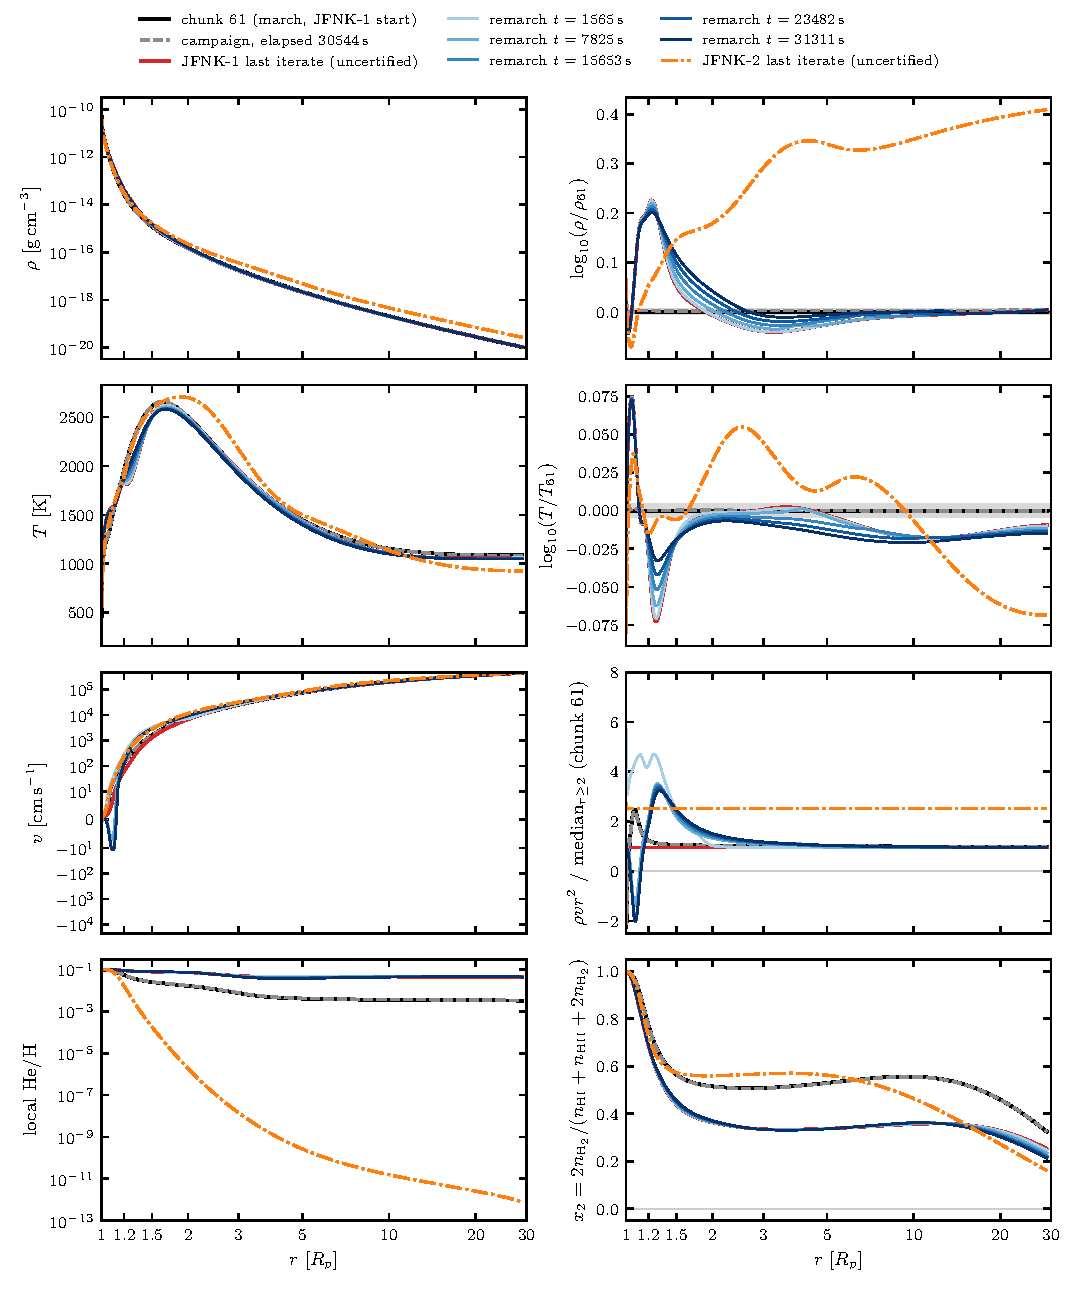
\includegraphics[width=\textwidth]{figures/jfnk_march_jfnk/fluid_profiles.pdf}
\caption{Fluid profiles. Black: chunk~61; gray dashed: campaign at elapsed
time 30\,544\,s; red: JFNK-1 last iterate (uncertified); blue (light to
dark): remarch at 1565, 7825, 15\,653, 23\,482 and 31\,311\,s; orange dash-dot: JFNK-2 last iterate (uncertified).
Right column: differences from chunk~61; the gray band is $\pm0.004$\,dex.
The mass flux is normalized by the median of chunk~61 over $r\ge2\,\Rp$.}
\label{fig:fluid}
\end{figure}

\section{A. The carriers when the JFNK-1 iterate is marched}\label{sec:a}

Figures~\ref{fig:carrratio}--\ref{fig:points} and
Table~\ref{tab:carr}. Two groups appear.

\textbf{Fast ions near the layer top (1.1--2\,$\Rp$).} Where the JFNK
carrier rows fail (cells 200--240, $r=1.15$--$1.30\,\Rp$), the JFNK-1
iterate carries more H$_2^+$, H$_3^+$ and HeH$^+$ than chunk~61 (up to
$+0.4$\,dex at 1.1--1.3\,$\Rp$ for H$_2^+$ and H$_3^+$, $+0.9$\,dex for
HeH$^+$). By the first frame (1564.5\,s) these fall by 0.40--1.03\,dex at
1.20--1.50\,$\Rp$, below the chunk-61 values, while at 1.27--2\,$\Rp$ He$^+$
and He(2$^3$S) rise by 0.16--0.36\,dex. The code itself quotes an H$_2^+$ lifetime of
about $10^{-3}$\,s (console, \texttt{molecular\_reaction\_heat}); with the
frames 1564.5\,s apart, we can only say that this change is present at
the first frame, which also includes the load re-equilibration
(Section~\ref{sec:setup}). Afterwards H$_2^+$ and HeH$^+$ partly rebound
($+0.30$ and $+0.43$\,dex at $1.27\,\Rp$, half of that change reached at
$\approx1.5\times10^{4}$\,s), apparently following the slower fluid change
below.

\textbf{Slow change in the layer (1.03--1.5\,$\Rp$).} H$^+$ and electrons
change by at most 0.12\,dex in the first frame and then steadily: at
$1.06\,\Rp$ H$^+$ falls by 0.75\,dex and $e^-$ by 0.49\,dex, at
$1.27\,\Rp$ both rise by 0.37--0.39\,dex; at these cells half of the
measured change is reached after 6000--8500\,s (at $1.50\,\Rp$ after
11\,500\,s); He(2$^3$S) at 1.03--1.1\,$\Rp$ falls by a further
0.24--0.47\,dex. Over the last chunk (23\,482--31\,311\,s) these quantities
still move by 0.01--0.06\,dex, so they have not settled. This is where the
velocity reverses sign in the remarch (inflow of up to 12\,cm\,s$^{-1}$ at
1.034--1.127\,$\Rp$, cells 117--191, at 31\,311\,s; outflow in chunk~61 and in JFNK-1;
Fig.~\ref{fig:fluid}).

\textbf{Wind ($r\ge3\,\Rp$) and neutrals.} Changes from the JFNK-1 iterate
are at most 0.34\,dex (He(2$^3$S) at $3\,\Rp$; He$^+$ 0.27\,dex there) and
below 0.2\,dex beyond $5\,\Rp$. H\,I, He\,I and H$_2$ change by at most
0.05, 0.06 and 0.08\,dex at any of the sampled cells. The helium excess of the JFNK
iterate is carried along: relative to the campaign at equal time, He\,I and
He$^+$ remain 0.7--1.06\,dex higher beyond $3\,\Rp$ throughout
(Fig.~\ref{fig:carrratio}).

By the first saved frame, the fast-ion densities have changed strongly
within the displaced fluid and helium distribution. They have not returned
to the chunk-61 values. By the end
of chunk~4 the stored state's carrier rows are $2.1\times10^{-3}$ to
$1.8\times10^{-2}$ (H$_2$ 0.109), as measured by JFNK-2 on load (its console
lines 130--151): far below the 0.5--0.85 the JFNK passes leave, though about
ten times the chunk-61 values ($9\times10^{-5}$ to $4.8\times10^{-3}$).

\begin{table}[!htbp]
\centering\small
\caption{Carrier changes in the remarch at selected cells
[\texttt{carrier\_timescales.txt}]: $\Delta_1$ = change of $\log_{10}n$ from the JFNK-1 iterate to the first frame (1564.5\,s),
$\Delta_2$ = change from the first frame to 31\,311\,s, $t_{1/2}$ = first time (interpolated between frames, measured from the remarch origin) at which half of the finite change $\Delta_2$ is reached;
it is not a chemical half-life or evidence of eventual equilibrium (for example, the small He(2$^3$S) change at cell 217 gives 1642\,s
despite later nonmonotonic changes). $\Delta_1$ includes the load re-equilibration.}
\label{tab:carr}
\begin{tabular}{rrlrrr}
\toprule
cell & $r$ [$\Rp$] & species & $\Delta_1$ [dex] & $\Delta_2$ [dex] & $t_{1/2}$ [s] \\
\midrule
149 & 1.060 & H$^+$ & -0.12 & -0.75 & 7597 \\
149 & 1.060 & H$_2^+$ & +0.11 & -0.42 & 6377 \\
149 & 1.060 & HeH$^+$ & +0.22 & -0.43 & 6574 \\
149 & 1.060 & He(2$^3$S) & -0.48 & -0.47 & 5929 \\
217 & 1.201 & H$^+$ & +0.02 & +0.04 & 4359 \\
217 & 1.201 & H$_2^+$ & -0.45 & +0.11 & 11517 \\
217 & 1.201 & HeH$^+$ & -0.64 & +0.16 & 12603 \\
217 & 1.201 & He(2$^3$S) & -0.02 & +0.00 & 1642 \\
234 & 1.270 & H$^+$ & +0.08 & +0.39 & 7343 \\
234 & 1.270 & H$_2^+$ & -0.65 & +0.30 & 14995 \\
234 & 1.270 & HeH$^+$ & -1.03 & +0.43 & 15122 \\
234 & 1.270 & He(2$^3$S) & +0.34 & +0.21 & 5264 \\
269 & 1.499 & H$^+$ & +0.05 & +0.40 & 11484 \\
269 & 1.499 & H$_2^+$ & -0.40 & +0.19 & 14803 \\
269 & 1.499 & HeH$^+$ & -0.61 & +0.19 & 15876 \\
269 & 1.499 & He(2$^3$S) & +0.36 & +0.30 & 10263 \\
309 & 2.003 & H$^+$ & +0.01 & +0.12 & 17139 \\
309 & 2.003 & H$_2^+$ & -0.18 & +0.01 & 19979 \\
309 & 2.003 & HeH$^+$ & -0.37 & +0.01 & 2690 \\
309 & 2.003 & He(2$^3$S) & +0.36 & +0.12 & 11367 \\
\bottomrule
\end{tabular}
\end{table}

\begin{figure}[!htbp]
\centering
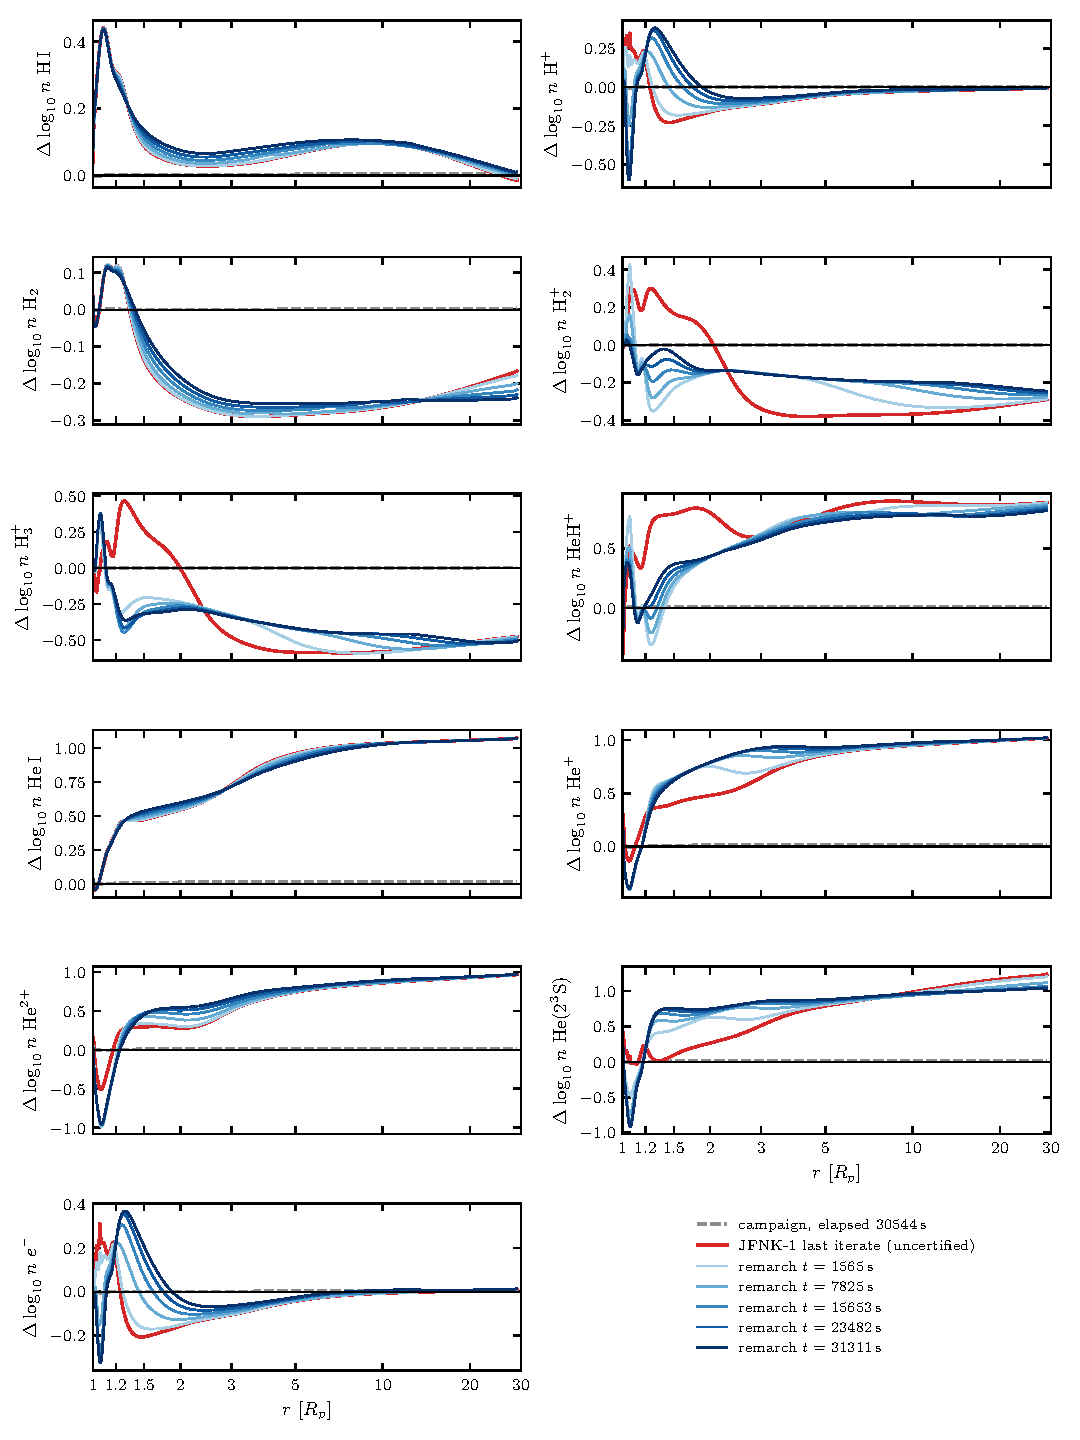
\includegraphics[width=\textwidth]{figures/jfnk_march_jfnk/carriers_ratio.pdf}
\caption{$\log_{10}$ of each density relative to chunk~61. Curves as in Fig.~\ref{fig:fluid}, without JFNK-2 (shown in Fig.~\ref{fig:j2}).}
\label{fig:carrratio}
\end{figure}

\begin{figure}[!htbp]
\centering
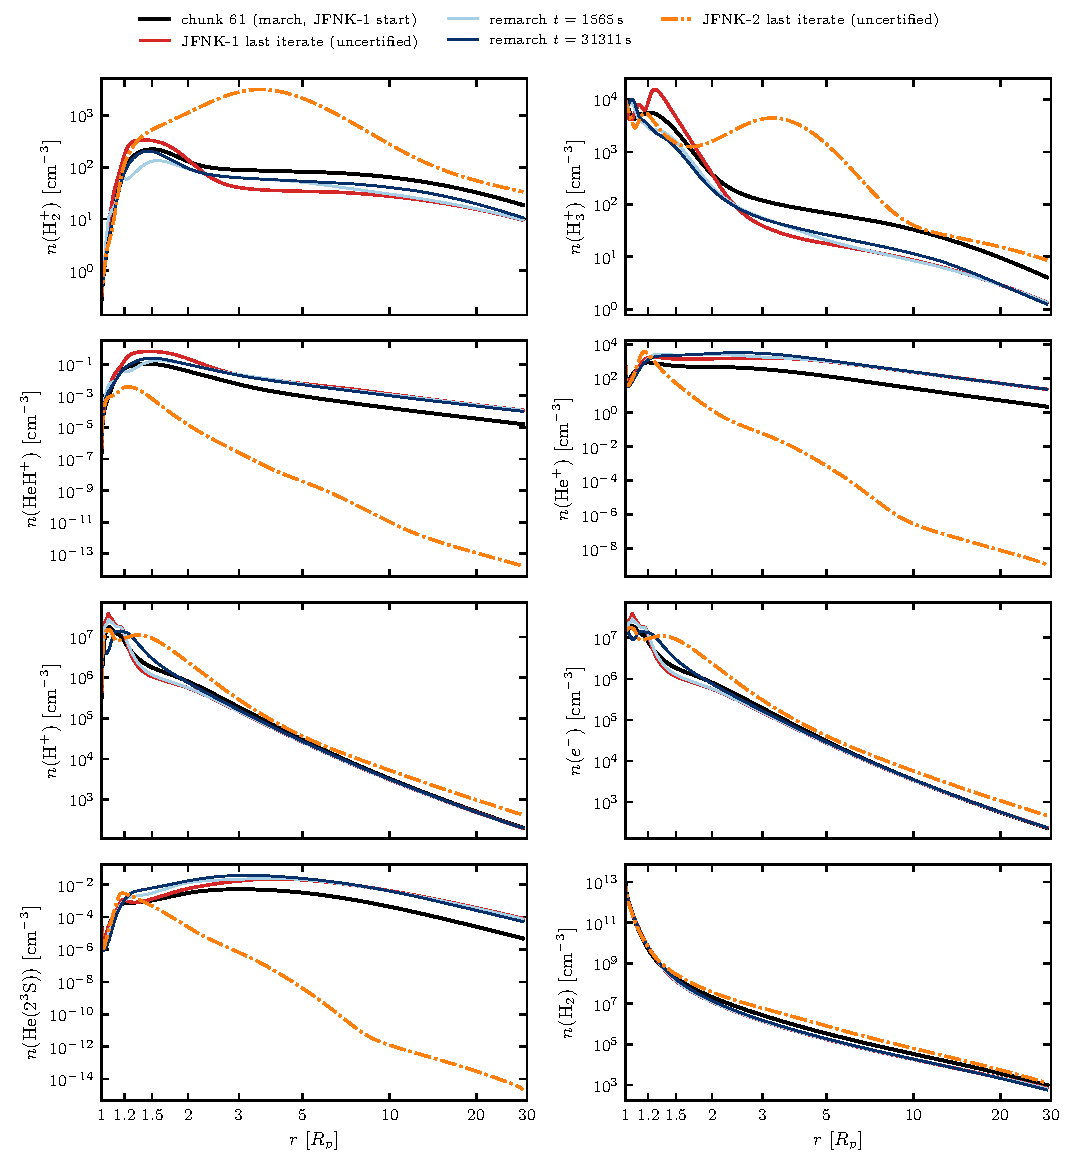
\includegraphics[width=\textwidth]{figures/jfnk_march_jfnk/carriers_abs.pdf}
\caption{Carrier and H$_2$ densities: chunk~61, JFNK-1 last iterate, the first and last remarch frames, and the JFNK-2 last iterate.}
\label{fig:carrabs}
\end{figure}

\begin{figure}[!htbp]
\centering
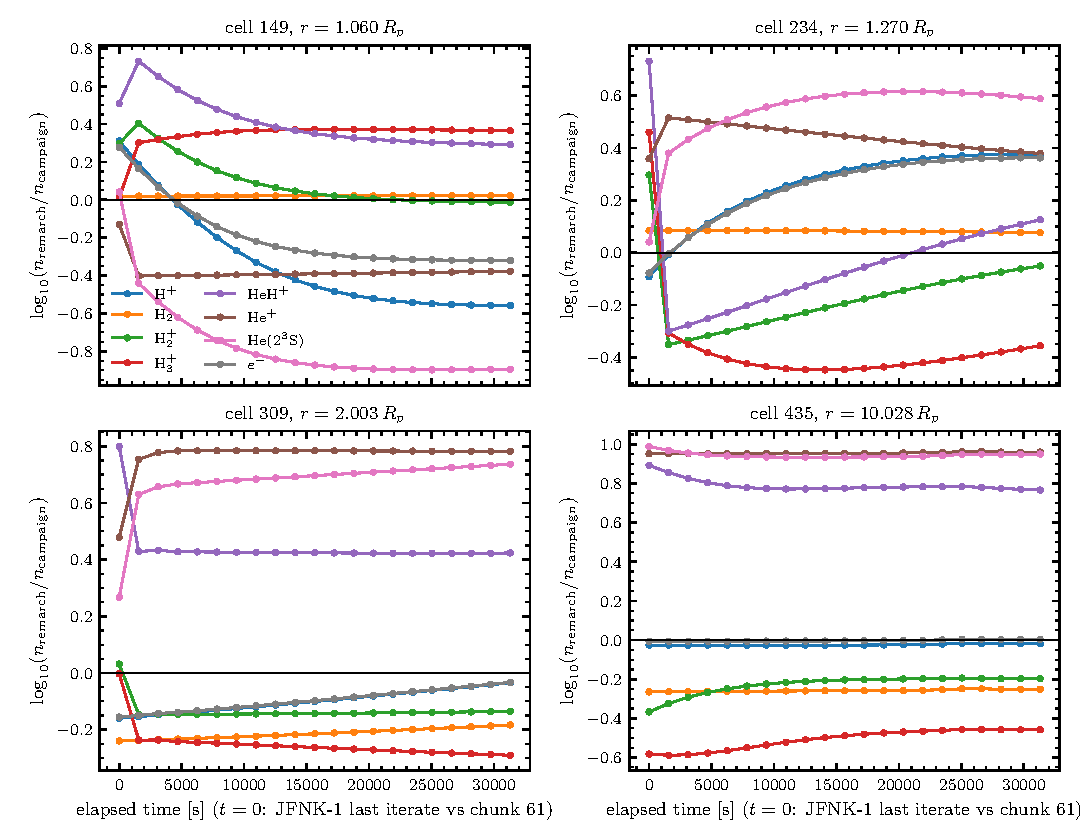
\includegraphics[width=\textwidth]{figures/jfnk_march_jfnk/carriers_points_time.pdf}
\caption{Remarch densities relative to the campaign at equal elapsed time, at four cells.
The point at $t=0$ is the JFNK-1 iterate relative to chunk~61; zero means the remarch
has returned to the campaign value.}
\label{fig:points}
\end{figure}

\section{B. The fluid: does it return to the marching state?}\label{sec:b}

\textbf{There is no overall return within 31\,311\,s} (0.106
$\tau_{\rm cross}$; Fig.~\ref{fig:dist}, Table~\ref{tab:dist}). The maximum
density and temperature differences decrease modestly, while the density
rms is nearly unchanged and the velocity difference grows. Against the campaign at equal
elapsed time, the largest $|\Delta\log_{10}\rho|$ goes from 0.226 (JFNK-1
vs chunk~61) to 0.225 at the first frame and 0.199 at 31\,311\,s, always at
$r=1.231\,\Rp$; its rms over the 500 cells stays at 0.082--0.083. The
largest $|\Delta\log_{10}T|$ goes from 0.075 to 0.071 (rms 0.035 to 0.031).
The $v$ measure grows from 0.087 to 0.33 at the first frame and 0.42 at
31\,311\,s; 434--461 cells stay outside the 0.004\,dex $\rho$ band and
389--489 outside the $T$ band. Over the same time the campaign moved from
chunk~61 by at most 0.0039\,dex in $\rho$, 0.0020\,dex in $T$ and 0.0013 in
$v$; the remarch moved away from the JFNK-1 iterate by 0.064\,dex in $\rho$
(at 1.54\,$\Rp$), 0.041\,dex in $T$ (at 1.27\,$\Rp$) and 0.52 in $v$.

\begin{table}[!htbp]
\centering\small
\caption{Distances over the 500 physical cells [\texttt{distance\_vs\_time.txt}].
$v$: the 1\% rule measure of \texttt{marching\_acceptance.velocity\_band} on the two-state set.
Limits: 0.004\,dex for $T$ and $\rho$, 0.01 for $v$.}
\label{tab:dist}
\begin{tabular}{lrrrrrr}
\toprule
pair & $t$ [s] & $\rho$ max (rms) [dex] & $T$ max (rms) [dex] & $v$ max (rms) & cells out $\rho$/$T$/$v$\\
\midrule
JFNK-1 $-$ chunk 61 & 0 & 0.2261 (0.0825) & 0.0746 (0.0349) & 0.087 (0.029) & 446/392/262 \\
remarch $-$ campaign & 1565 & 0.2251 (0.0826) & 0.0745 (0.0347) & 0.332 (0.093) & 448/389/264 \\
remarch $-$ campaign & 7825 & 0.2198 (0.0824) & 0.0738 (0.0338) & 0.339 (0.105) & 452/403/262 \\
remarch $-$ campaign & 15653 & 0.2127 (0.0824) & 0.0729 (0.0327) & 0.386 (0.112) & 461/475/270 \\
remarch $-$ campaign & 23482 & 0.2057 (0.0825) & 0.0720 (0.0319) & 0.409 (0.116) & 459/489/252 \\
remarch $-$ campaign & 31311 & 0.1993 (0.0830) & 0.0712 (0.0313) & 0.420 (0.117) & 434/489/249 \\
remarch $-$ JFNK-1 & 1565 & 0.0035 (0.0010) & 0.0021 (0.0005) & 0.391 (0.111) & 0/0/131 \\
remarch $-$ JFNK-1 & 31311 & 0.0638 (0.0247) & 0.0406 (0.0103) & 0.515 (0.129) & 274/232/228 \\
campaign $-$ chunk 61 & 30544 & 0.0037 (0.0023) & 0.0019 (0.0006) & 0.001 (0.001) & 0/0/0 \\
\bottomrule
\end{tabular}
\end{table}

\textbf{Where the change happens.} In $\rho$ and $T$ the remarch change is
gradual: 0.0035\,dex in $\rho$ and 0.0021\,dex in $T$ at the first frame,
growing to 0.064 and 0.041\,dex at 31\,311\,s at an almost constant rate
(Fig.~\ref{fig:dist}). In $v$, 0.39 of the final 0.52 is present at the
first frame. The mass-flux spread $du$ over $r\ge2\,\Rp$ rises from
$2.3\times10^{-4}$ (the JFNK-1 iterate) to $7.7\times10^{-2}$ at step
10\,000, peaks at 0.583 at step 16\,920 of chunk~1 (about 2640\,s, a time
interpolated between saved clocks), and then grows slowly from 0.31 to
0.52. For campaign chunks 62--65, $du$ decreases from 0.05565 to 0.05378.
The relative change of the conserved state over one step,
$dtu=\max|1-u/u_{\rm old}|$ (EXHALE\_main.f90 3556--3583; not a stationary
residual), peaks at $1.0065\times10^{-4}$ (chunk~1, step 12\,619) in the raw
remarch sequence and reaches $1.2681\times10^{-6}$ at chunk~4 step 50\,000
and $6.3406\times10^{-7}$ at step 50\,001; campaign values at step 50\,000
remain near 4.4--$4.5\times10^{-8}$. The excess mass flux
sits at 1.05--2\,$\Rp$: at 31\,311\,s, $\rho v r^2$ is $-2.0$ to $+3.2$
times the chunk-61 median at 1.05--1.5\,$\Rp$, with inflow at
1.034--1.127\,$\Rp$; $4\pi\rho v r^2$ at cell $N-20$ stays at
$7.08\times10^7$\,g\,s$^{-1}$ (campaign $7.35\times10^7$). A density excess
travels outward from 1.5 to about 3\,$\Rp$ during the four chunks
(Fig.~\ref{fig:fluid}).

\textbf{Time scales.} From the states we evaluate
$\tau_{\rm cross}=2.91$--$3.35\times10^5$\,s (flow crossing beyond Mach
0.01; \texttt{marching\_acceptance.crossing\_times}) and a sound crossing of
the whole domain $\sum\Delta r/(c_s+|v|)=5.84\times10^{4}$\,s; 31\,311\,s
is 0.106\,$\tau_{\rm cross}$ and 0.54 sound-crossing times. The advection
time $\sum\Delta r/|v|$ is $2.3\times10^6$\,s over 1.1--1.2\,$\Rp$,
$8.3\times10^5$\,s over 1.2--1.5\,$\Rp$, $1.7\times10^5$\,s over
1.5--2\,$\Rp$ and $2.6\times10^5$\,s over 2--30\,$\Rp$ in chunk~61
[\texttt{segment\_times.txt}]. A difference that does not decay within
the march is the helium distribution of the layer below 2\,$\Rp$ (He/H at
1.2--2\,$\Rp$ changes by at most 0.0011, 1.5\%, in the remarch, and in the
direction away from chunk~61). The campaign
itself drifts toward more helium: its He/H at $1.2\,\Rp$ rises from
0.05295 to 0.05384 between elapsed $-22\,554$ and $+25\,747$\,s
(0.0072\,dex), at $10\,\Rp$ by 0.018\,dex. If these slopes of
$\log_{10}$(He/H) were held constant, the campaign would reach the JFNK-1
ratios at 1.2 and $10\,\Rp$ after about $1.4\times10^6$ and
$3.0\times10^6$\,s, or 5 and 10 chunk-61 crossing times; a constant slope
of the ratio itself would instead give $1.8\times10^6$ and
$1.4\times10^7$\,s. These are illustrative extrapolations of a short record,
not predictions, lower bounds of the return time of the remarch, or
acceptance conditions. The rms $\rho$ distance of the remarch shows no
decrease. The remarch does not return to the campaign state within the
measured 0.106 crossing times; the different helium distribution and the
long advection times are consistent with persistence of the disturbance,
but these runs do not establish its cause or its eventual relaxation time.
These stationary diagnostics and the helium drift do not change the
campaign's marching acceptance criterion (the T, $\rho$ and $v$ bands over
the final $K=3$ crossing-time window); they add no required waiting time.

\begin{figure}[!htbp]
\centering
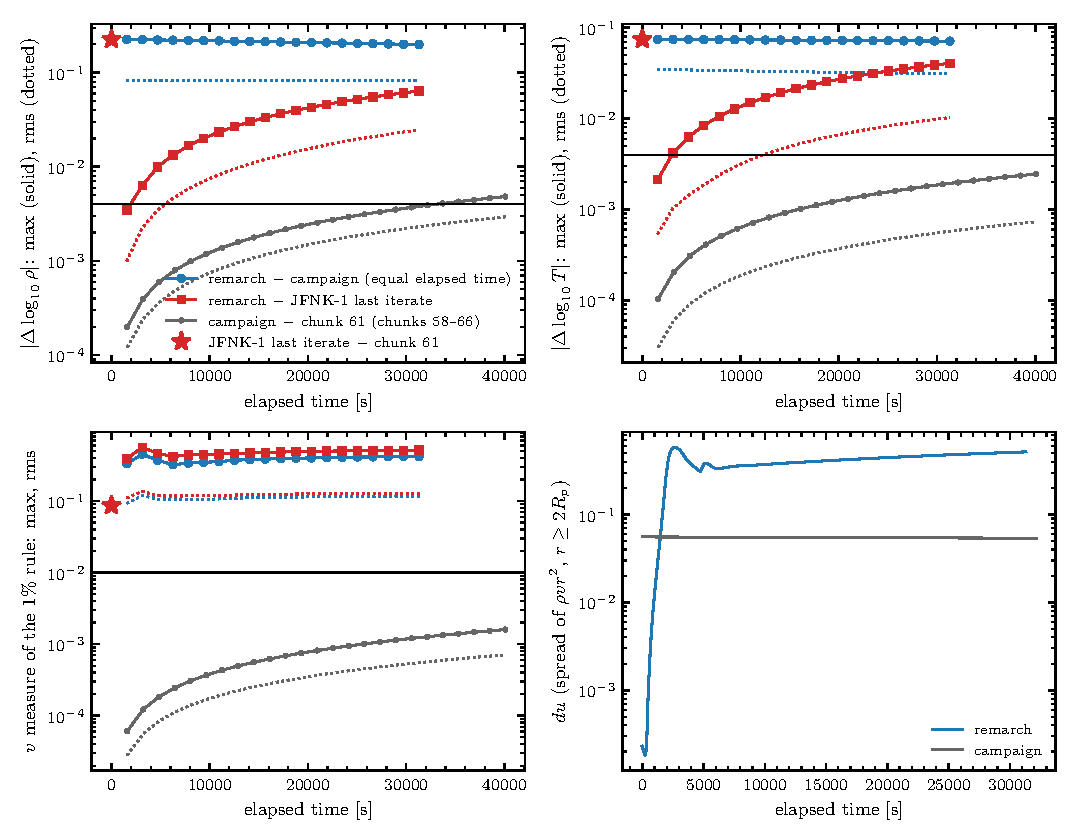
\includegraphics[width=\textwidth]{figures/jfnk_march_jfnk/distance_time.pdf}
\caption{Distances in time. Blue: remarch against the campaign at equal
elapsed time; red: remarch against the JFNK-1 iterate; gray: campaign
against chunk~61; star: JFNK-1 iterate against chunk~61. Solid: maximum over
cells; dotted: rms. Horizontal lines: the 1\% limits. Lower right: $du$
from the console records of every step (remarch, campaign chunks 62--65).}
\label{fig:dist}
\end{figure}

\section{C. JFNK-2 compared with JFNK-1}\label{sec:c}

\textbf{Pass histories} (Fig.~\ref{fig:passes};
\texttt{outer\_passes\_jfnk\{1,2\}.txt}). Both attempts used all 60 passes
with \texttt{info=1}. Hydrodynamic \texttt{info=0} in every pass except
6, 49, 51 (JFNK-1) and 7 (JFNK-2). In these passes, \texttt{info=2} caused
the failed hydrodynamic iterate to be discarded and the last converged wind
and its composition to be restored (EXHALE\_main.f90 8148--8164); the
composition update was then recomputed with $\omega=0.5$ and a reduced
carrier movement bound (8660--8669), and the next hydrodynamic solve
occurred in the following outer pass. Wall time per pass over all 60
passes: median 263.975 and 264.125\,s, mean 331.849 and 268.903\,s; JFNK-1 had six passes above 700\,s (passes 5, 6, 7, 56, 57, 59),
JFNK-2 none above 400\,s. JFNK-2 ran on lart3 with
load average 23.4 at its start (JFNK-1: 12.1).

\textbf{The two starts lead to similar late-pass diagnostics.} JFNK-2 started from
a state whose carrier rows were $2.1\times10^{-3}$--$1.8\times10^{-2}$
(JFNK-1: $9\times10^{-5}$--$4.8\times10^{-3}$) and whose He/H already had the
JFNK-1 distribution. Its first worst row was 0.71 (JFNK-1: 0.40), and it had
no approach phase: 0.48--0.64 in passes 2--8 against 0.08--0.17 for
JFNK-1 in passes 2--6. At passes 28--35 the worst rows of the two attempts differ by up to
0.065 and the worst cells by up to 59. From pass~36 to pass~48 the
records are similar: the same worst species, cells within two of each
other, worst rows within 0.03, similar element and carrier displacements
(e.g.\ pass~37 carrier displacement 0.333 and 0.353), and the same kind of
ending of the carrier update (e.g.\ pass~40: He(2$^3$S) at cell 500, 0.998
in both; pass~45: H$_2^+$ at cell 343, 0.836 and 0.835). JFNK-2 passes
49--59 resemble its passes 32--42 in the printed diagnostics (largest
difference of the worst row 0.007, same species); this is not an exact
repeat of all entries (pass 35 against 52: worst cell 365 against 309) or a
comparison of full states. JFNK-1 departs from the similar diagnostic
sequence at pass~49 (\texttt{info=2}).

\textbf{Where the JFNK-2 last iterate lies} (Fig.~\ref{fig:j2};
\texttt{jfnk2\_compare.txt}; maxima over cells, rms in brackets).
\begin{center}\small
\begin{tabular}{lccc}
\toprule
pair & $\rho$ [dex] & $T$ [dex] & $v$ measure \\
\midrule
JFNK-2 $-$ its start (remarch end) & 0.406 (0.219) at $28.5\,\Rp$ & 0.062 & 0.23 \\
JFNK-2 $-$ JFNK-1 & 0.405 (0.231) at $28.5\,\Rp$ & 0.066 & 0.79 \\
JFNK-2 $-$ chunk 61 & 0.409 (0.216) at $29.0\,\Rp$ & 0.081 & 0.65 \\
JFNK-1 $-$ chunk 61 & 0.226 (0.082) at $1.23\,\Rp$ & 0.075 & 0.09 \\
\bottomrule
\end{tabular}
\end{center}
JFNK-2 removes helium from the wind: He/H is 0.0154 at $1.2\,\Rp$,
$1.8\times10^{-4}$ at $1.5\,\Rp$, $1.8\times10^{-6}$ at $2\,\Rp$ and
$1.5\times10^{-11}$ at $10\,\Rp$, against 0.0875, 0.078, 0.072 and 0.045 in
JFNK-1 and 0.053, 0.025, 0.017 and 0.0035 in chunk~61. Its $x_2$ at
2--5\,$\Rp$ (0.56--0.57) is close to chunk~61 (0.51--0.53), unlike JFNK-1
(0.34--0.36). Its density is 0.18--0.29\,dex higher than chunk~61 at 2--3\,$\Rp$ and
0.29--0.41\,dex higher beyond $3\,\Rp$, and its
$4\pi\rho v r^2$ at cell $N-20$ is $1.869\times10^{8}$\,g\,s$^{-1}$, 2.6 times
chunk~61 ($7.28\times10^7$) and JFNK-1 ($7.08\times10^7$), with spread
$du=1.8\times10^{-4}$.

\textbf{Is the displacement reproducible?} Not as a state. Over the 500
cells, the JFNK-2 displacement (JFNK-2 minus its start) is
\emph{anti}-correlated with the JFNK-1 displacement (JFNK-1 minus chunk~61):
Pearson coefficient $-0.60$ in $\log\rho$, $-0.48$ in $\log T$, $-0.99$ in
$\log$ He/H. The march between them returned almost nothing of the JFNK-1
displacement: the least-squares slope of the march change on the JFNK-1
displacement is $-0.024$ in $\log\rho$ and $-0.13$ in $\log T$.
What recurs is a similar late-pass diagnostic record and a large
helium contrast between the two saved pass states of each attempt
(Section~\ref{sec:d}): the JFNK-1 last iterate is helium-rich, the JFNK-2
last iterate helium-poor. The
kept states of the same phase from the two attempts are closer to each
other than to the opposite phase: the two helium-rich states (JFNK-1
\texttt{\_p59}, JFNK-2 \texttt{\_p58}) differ by 0.22\,dex in $\rho$,
0.068\,dex in $T$ and 0.16\,dex in He/H, while consecutive states of one
attempt differ by 0.89 (JFNK-1) and 1.66\,dex (JFNK-2) in $\rho$. The saved states and scalar diagnostics appear consistent with a strongly
varying partitioned iteration that does not approach the marching state.
They do not establish a common periodic orbit or an alternative stationary
solution.

\begin{figure}[!htbp]
\centering
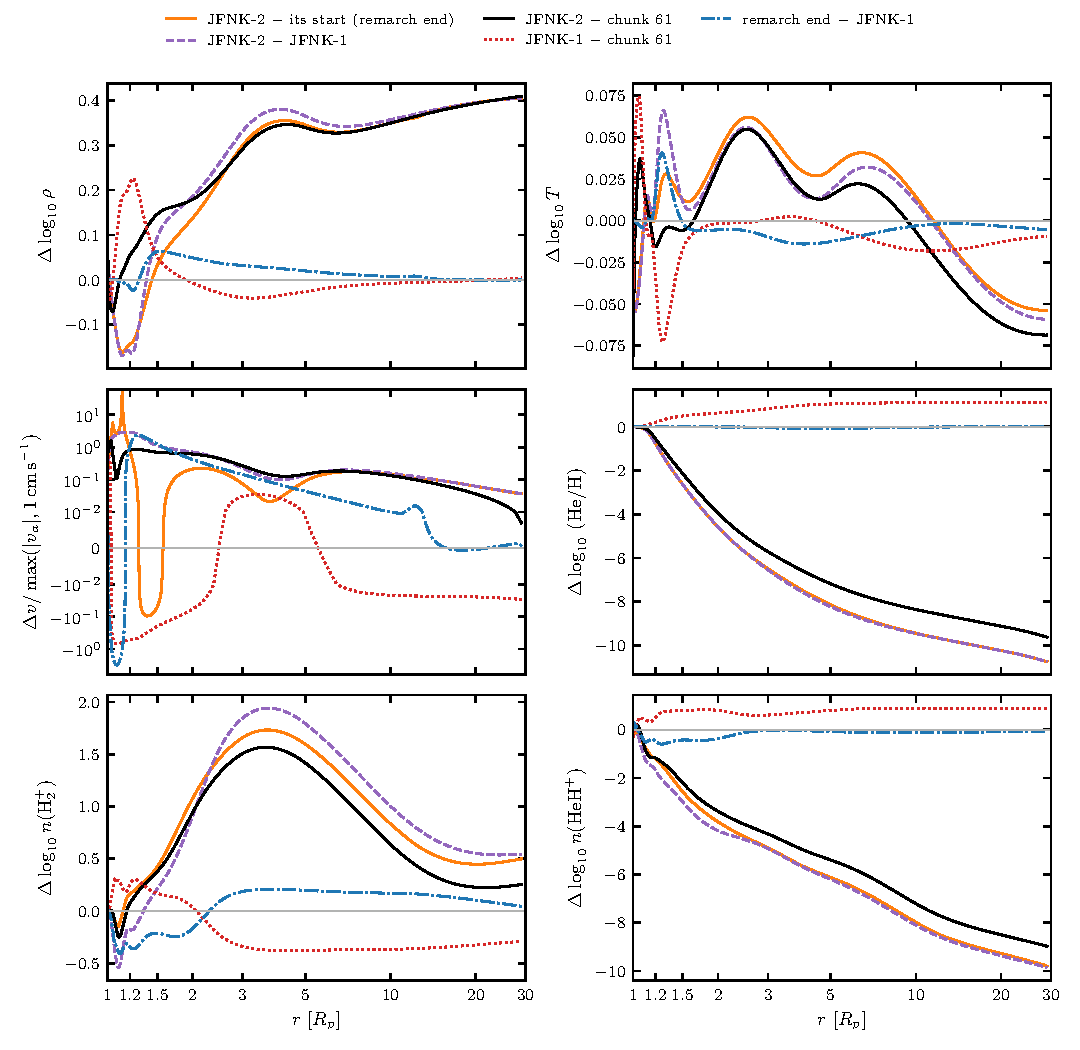
\includegraphics[width=\textwidth]{figures/jfnk_march_jfnk/jfnk2_compare.pdf}
\caption{Cellwise differences between the JFNK-2 last iterate, its start
(the end of the remarch), the JFNK-1 last iterate and chunk~61. The
velocity panel shows $\Delta v/\max(|v_a|,1\,{\rm cm\,s^{-1}})$, $a$ the
reference state of each pair, on a symmetric logarithmic scale.}
\label{fig:j2}
\end{figure}

\section{D. How the state moves during the outer passes}\label{sec:d}

\textbf{What is kept.} Each attempt publishes the state after the
composition update of a pass into \path{output/pass_state/} and keeps only
the last two: JFNK-1 holds \texttt{\_p58} and \texttt{\_p59} (both
complete, with manifest, Hydro, Ion and conserved files; \texttt{current}
names \texttt{\_p59}, which is not empty when read on 2026-11-12),
and JFNK-2 holds \texttt{\_p58} and \texttt{\_p59}.
Earlier pass states are not available, so the motion over the passes is
read from the console lines of each pass (Table files
\texttt{outer\_passes\_jfnk\{1,2\}.txt}, Fig.~\ref{fig:passes}).

\textbf{JFNK-1, passes 1--8: an approach.} The first element relaxation
reports a displacement of 0.549; the following element displacements fall to
0.035--0.09 (passes 4--8), the carrier updates are limited by the trust
radius, which doubles from 0.01 to 0.16, and the worst carrier row after
the hydrodynamic solve falls from 0.40 to 0.08 (passes 5--6; H$_2^+$ at
cell 243, $1.32\,\Rp$).

\textbf{Passes 9--60: no further approach; a recurring pattern of pass types.} At pass 9 the
element relaxation stops on its step budget with a displacement of 0.87,
and from then on the worst row stays at 0.42--1.0. From pass 19 a pattern
recurs every 2--4 passes: a pass whose carrier relaxation ends because the
shortest admissible trial interval was not covered, with a carrier
displacement of 2.5--2.7 and the worst carrier residual in He$^{2+}$ at
8--29\,$\Rp$; then a pass with composition under-relaxation $\omega=0.5$
ending on the movement bound (displacement 0.97); then one or two passes
ending on the step budget, whose returned carrier residual is
$5\times10^{-5}$--$5\times10^{-4}$. In passes 38--46 the element
relaxation applies 0.88--0.91 in every pass, alternating between the two
kinds of carrier update. The worst row sits in two groups of cells: 200--243
($1.15$--$1.32\,\Rp$, mostly H$_2^+$, HeH$^+$) and 278--357
($1.58$--$3.32\,\Rp$, mostly He$^+$, H$_2^+$), with He(2$^3$S) at the outer
boundary (cells 426--500) in passes 40, 42, 44. The hydrodynamic solve
returned \texttt{info=2} in passes 6, 49 and 51; each failed iterate was
discarded and the composition update was recomputed from the restored
converged wind with $\omega=0.5$. It returned \texttt{info=0} otherwise. The H$_2$ ``front''
printed by the code (innermost cell with $x_2<0.5$) jumps between 1.23 and
22.6\,$\Rp$ because $x_2$ stays near 0.5 over most of the wind; it is not a
useful position measure here.

\textbf{The size of the change between passes.} The two kept JFNK-1 states differ
enormously: wind He/H is $3.8$--$5\times10^{-8}$ beyond $10\,\Rp$ in
\texttt{\_p58} and 0.044--0.045 in \texttt{\_p59}; $\rho$ differs by up to
0.89\,dex ($4.2\,\Rp$), $T$ by 0.17\,dex and the $v$ measure by 0.47.
The step from \texttt{\_p59} to the final iterate (the hydrodynamic solve
of pass~60 with its usual thermochemical and boundary refreshes, no element
or carrier update; He/H changes by less than $2\times10^{-14}$\,dex) moves $\rho$ by up to 0.23\,dex, $T$ by
0.13\,dex and $v$ by 0.33 (Fig.~\ref{fig:passstates}). The final iterate of an attempt thus appears to be one state of a
strongly varying sequence, not the end of a drift. Two adjacent saved states
cannot establish a sustained alternation of full profiles, a periodic
orbit, or independence from the initial state; they show that adjacent
passes moved the state by more than the JFNK-1 to chunk-61 difference.
In JFNK-2 the two kept states are the other way round: \texttt{\_p58} is
helium-rich (He/H 0.064 at $10\,\Rp$) and \texttt{\_p59} helium-poor
($1.5\times10^{-11}$); they differ by 1.66\,dex in $\rho$ and 0.27\,dex in
$T$, and the hydrodynamic solve of pass~60 moves $\rho$ by 1.62\,dex. The
mass-loss measure $4\pi\rho v r^2$ at cell $N-20$ of the kept states is
$2.1\times10^7$ and $1.22\times10^8$\,g\,s$^{-1}$ (JFNK-1 \texttt{\_p58},
\texttt{\_p59}) and $2.07\times10^8$ and $8.5\times10^6$\,g\,s$^{-1}$
(JFNK-2), i.e.\ it changes by a factor 6--24 from one pass to the next.

\begin{figure}[!htbp]
\centering
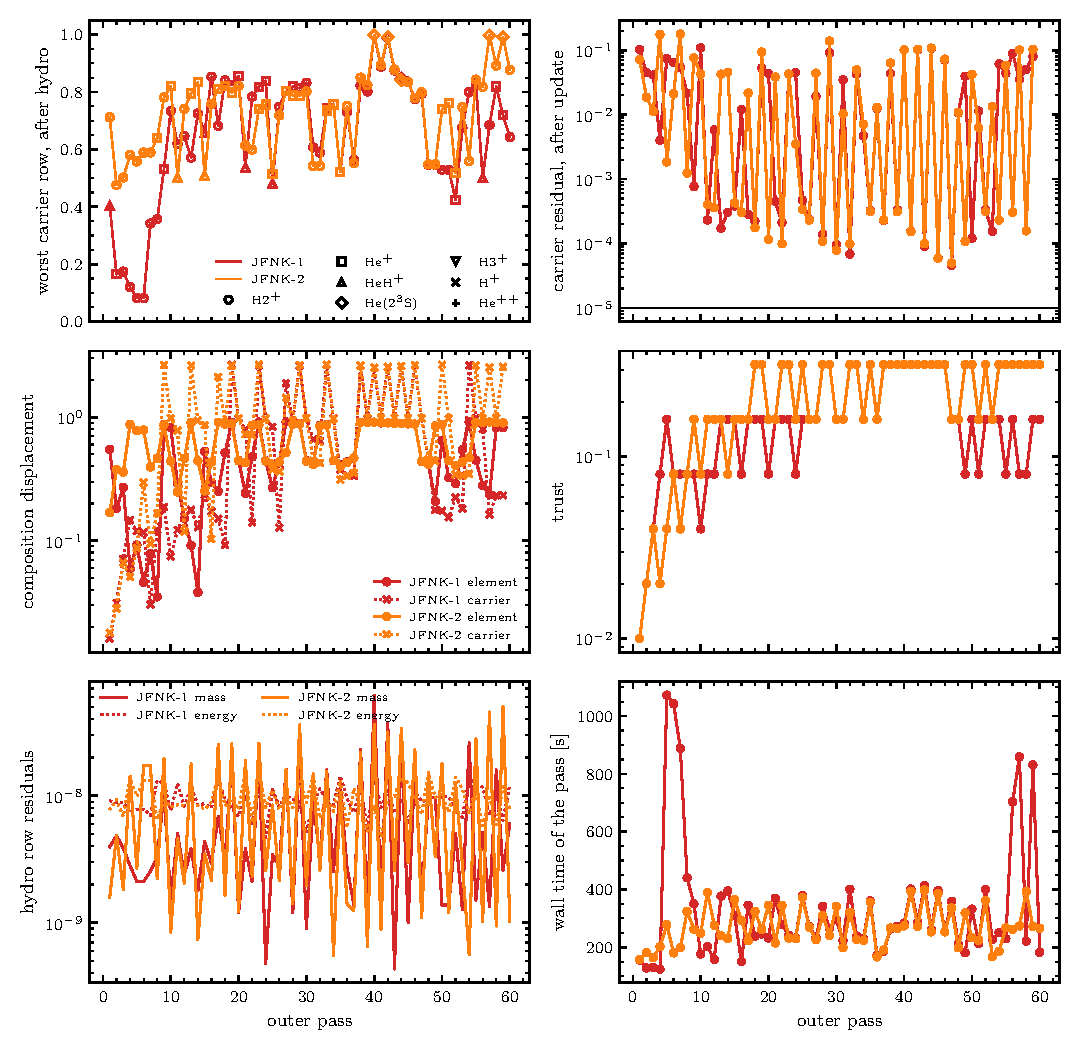
\includegraphics[width=\textwidth]{figures/jfnk_march_jfnk/outer_passes.pdf}
\caption{Outer-pass histories of JFNK-1 (red) and JFNK-2 (orange). Upper
left: worst gated carrier row after the hydrodynamic solve (transported
fractions retained, with the usual thermochemical and boundary refreshes),
with the species; upper right: carrier residual of the composition returned by the
update of the pass (horizontal line: $10^{-5}$); middle: element and
carrier displacements and the trust radius; lower: hydrodynamic row
residuals and wall time of each pass.}
\label{fig:passes}
\end{figure}

\begin{figure}[!htbp]
\centering
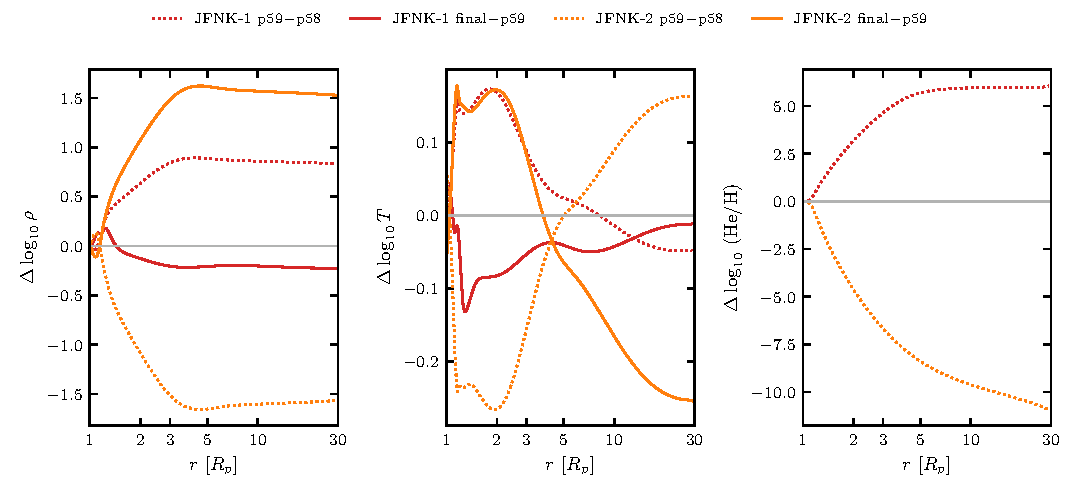
\includegraphics[width=\textwidth]{figures/jfnk_march_jfnk/pass_states.pdf}
\caption{Motion between the saved intermediate iterates. Dotted:
\texttt{\_p59} minus \texttt{\_p58} (one hydrodynamic solve and one
composition update). Solid: the uncertified last iterate minus
\texttt{\_p59} (the final hydrodynamic solve with its usual thermochemical
and boundary refreshes, without a subsequent element or carrier update).}
\label{fig:passstates}
\end{figure}

\section{E. Why the carrier rows do not close: a cautious reading}\label{sec:e}

\textbf{What the row is.} The carrier balance entry of the certification
is, for each transported carrier and cell, the stationary form of its
transport equation: the divergence of its diffusive, eddy and drift face
fluxes, plus the divergence of its advective face flux, minus the net
chemical source, with the time term removed ($\Delta t=10^{30}$)
(\texttt{carrier\_steady\_residual} and \texttt{carrier\_residual},
\path{diffusive_photochemistry.f90} 4288--4525, 7402--7535). It is normalized
by the sum of the absolute diffusive face contributions, the advective
magnitude, the gross chemical production and loss, and an absolute floor
(7417--7425, 7453, 7503, 4491). The floor is $10^{-20}$ times a
carrier-specific elemental reference density (free hydrogen for H$_2$,
H$^+$, H$_2^+$, H$_3^+$; total helium nuclei for the helium stages and
He(2$^3$S); the smaller of the two for HeH$^+$; 5771--5804) times the
cell's signal-crossing rate. The tolerance is $10^{-5}$. A measure
$q=0.5$--0.85 represents an imbalance of 50--85\% of that sum. Only when
transport and the floor are negligible is $q=|P-L|/(P+L)$, implying
$\max(P,L)/\min(P,L)=(1+q)/(1-q)$, about 3--12.3. The corresponding
volume-weighted measures are also large; pass~30 of JFNK-1 gives 0.54,
0.33 and 0.44 for He$^+$, H$_2^+$ and HeH$^+$
[\texttt{handed\_back\_rows\_jfnk1.txt}]. These integrated measures do
not by themselves determine the number or radial extent of the affected
cells.

\textbf{What the records show.}
\begin{enumerate}
\item In marching states these rows are much smaller, though still above
$10^{-5}$: $9.3\times10^{-5}$--$4.8\times10^{-3}$ in chunk~61 (H$_2$ 0.15 at
cell~3), $2.1\times10^{-3}$--$1.8\times10^{-2}$ at the end of the remarch
(H$_2$ 0.11).
\item Inside the JFNK passes, the composition updates reduce the maximum
carrier residual to $4.6\times10^{-5}$--$3.3\times10^{-4}$ in the listed
step-budget-limited passes, while remaining above the $10^{-5}$ stationary
tolerance (JFNK-1 passes 30, 32, 39, 41, 43, 45, 47; Fig.~\ref{fig:passes}).
\item The next hydrodynamic solve, with the transported fractions retained
(console line 29: ``hydrodynamic sweeps retain transported x(H\,II),
x(He\,II) and x(He\,III)'') and the usual thermochemical and boundary
refreshes applied (EXHALE\_main.f90 8043--8080), raises the worst gated
carrier residual to 0.55--1.0 in the listed passes (31, 33, 40, 42, 44,
46, 48 of JFNK-1). The transition from the saved pass-59 state to the
uncertified last iterate contains this hydrodynamic solve and its
refreshes, with no subsequent element or carrier relaxation; in it $T$
changes by up to
0.13\,dex ($1.30\,\Rp$), $\rho$ by up to 0.23\,dex, and $v$ at
$1.26\,\Rp$ by $-61\%$ in JFNK-1; in JFNK-2 the same step changes $T$ by up
to 0.25\,dex and $\rho$ by up to 1.62\,dex.
\item The helium partition does not settle: the element relaxation applies
a displacement of 0.88--0.91 in every pass from 38 to 46, and the two
published pass states of JFNK-1 have wind He/H of $4\times10^{-8}$ (pass
58) and 0.045 (pass 59) (Section~\ref{sec:d}).
\end{enumerate}

\textbf{Reading (tentative).} The records appear consistent with a
partitioned iteration that does not contract: a hydrodynamic solve with
retained transported fractions changes $T$ and $\rho$ by 0.1\,dex or more
(the two solves that can be isolated, pass~60 of each attempt), which
might be enough to unbalance the fast ions by an $O(1)$ fraction of their
gross rates; each composition update then moves helium and the carriers by
amounts that change the next hydrodynamic solution by a similar amount.
This is not a term-by-term causal proof. The march instead advances the
coupled time-dependent model with its existing operator splitting and small
physical steps of about 0.16\,s, far shorter than the
$\sim10^4$\,s on which the layer evolves, and the fast-carrier rows stay much
smaller (though above $10^{-5}$). We have not decomposed the rows into their terms (the row-term
record \texttt{EXHALE\_CARRIER\_ROW\_TERMS} was off), so which term
(production, loss or transport) carries the imbalance in the named cells is
not measured. Two consequences can be stated from the measurements alone:
(i) with the present route and settings, a JFNK last iterate of this
molecular case is not a stationary state of the carrier and helium
equations and lies outside the 1\% band of the marching state; (ii)
marching from such an iterate did not return to the marching state within
0.1\,$\tau_{\rm cross}$; the different helium distribution in a layer whose
advection times exceed $10^6$\,s is consistent with that persistence, but
the runs do not establish its cause. Using a JFNK iterate as a start for
further marching would therefore introduce a disturbance of unknown
relaxation time. The
campaign state itself is not stationary in He/H either (normalized
elemental residual 0.31 at cell~4; He/H rising slowly, Section~\ref{sec:b}); which helium
distribution the stationary wind has is not decided by these runs.

\section*{Not checked}
\begin{itemize}
\item The composition change made by the load re-equilibration of remarch
chunk~1, species by species: no state is written before step 10\,001.
\item Carrier changes faster than the frame interval of 1564.5\,s; the
fast-ion time scale is the code's own quoted H$_2^+$ lifetime, not a
measurement here.
\item The individual terms (production, loss, transport) of the
unbalanced carrier rows; the row-term record was off in all runs.
\item The states of JFNK passes other than the last two of each attempt.
\item Whether the remarch would return to the campaign state over one or
more crossing times; only 0.106\,$\tau_{\rm cross}$ was marched, and the
statements on longer times are illustrative extrapolations of
$\log_{10}$(He/H), not predictions or bounds.
\item Which helium distribution (the marching one or the JFNK one) the
stationary wind has; neither state is certified and the normalized
elemental He/H residual of the marching state is 0.31.
\item The physical acceptability of the remarch inflow at
1.03--1.13\,$\Rp$ and of the pass-to-pass variation of the JFNK iterates; no
resolution, CFL or step-size test was made.
\item Bitwise or host effects: the campaign ran on lart1, the remarch and
both JFNK attempts on lart3; no replay was made.
\item The decomposition of the remaining 0.2\,dex density difference at
$1.23\,\Rp$ into composition (mean molecular mass) and structure.
\item Mdot from \texttt{EXHALE\_resolved.out} of each state; we quote
$4\pi\rho v r^2$ at cell $N-20$ computed from the profiles.
\end{itemize}

\section*{Sources}
Paths relative to \path{EXHALE_v1.10/}; $E$ = \path{scratch_jfnk_from_marching_20261111/heh0p1_s2p53/},
$P$ = \path{LHS1140b/models/marching_campaign_he01_series_20261106/cases/heh0p1_s2p53/phase/}.
\begin{itemize}
\item R1: $E$\path{run/} (\path{console.log}, \path{VERDICT.txt}, \path{EXIT.txt}, \path{output/}); PLAN: $E$\path{PLAN.txt};
remarch plan $E$\path{remarch/PLAN.txt}.
\item RJ: $E$\path{remarch/journal.txt}, \path{progress.txt}, \path{chunks/c000k/console.log}.
\item R2: $E$\path{remarch/jfnk2/run/}; CP: $P$\path{progress.txt}, $P$\path{journal.txt}, $P$\path{snapshots/}, $P$\path{chunks/c006k.log.gz}.
\item T: tables and scripts in $E$\path{remarch/analysis/} (\path{ana_common.py}, \path{march_analysis.py},
\path{du_series.py}, \path{carrier_timescales.py}, \path{outer_passes.py}, \path{jfnk2_compare.py}, \path{figures.py});
readers \path{examples/exhale_io.py} and \path{LHS1140b/tools/marching_acceptance.py}.
\item Source code: \path{src/EXHALE_main.f90} (step record 4194, \texttt{mass\_flux\_spread} 4968--4995,
H$_2$ front 9380--9420); \path{src/modules/lower_atmosphere/diffusive_photochemistry.f90}
(\texttt{carrier\_steady\_residual} 4288--4525, \texttt{carrier\_residual} 7170--7565);
\path{src/modules/time_step/certification.f90} (carrier entries 1898--2200).
\end{itemize}

\end{document}
